\documentclass[../zhang_thesis.tex]{subfiles}
\begin{document}

\chapter{Methodology}

%%%%%%%%%%%%%%%%%%%%%%%%%%%%%%%%%%%%%%%%%%%%%%%%%%%%%%%%%%%%%%%

\section{Battery Model}

As discussed in the previous section, this thesis considers the electrical-circuit battery model proposed by Chen and Rinc\'on-Mora~\cite{chen06} and shown in \autoref{fig:batt_model}. The left portion of the circuit models the capacity, SOC, and runtime, while the right portion models the transient i-v characteristics.  For convenience, the model is designed so that the SOC of the battery equals the voltage $V_\text{SOC}$, in volts. The parameters $C_\text{cap}$ and $R_{sd}$ are assumed constant
for a given battery and determine the capacity and self-discharge rate of the battery. The other parameters are all nonlinear functions of $V_\text{SOC}$ and determine the transient i-v response as well as the open-circuit voltage $V_\text{OC}$. From a typical TCL PL-383562 polymer lithium-ion battery, Chen and Rinc\'on-Mora extracted these parameters and fit them to curves, obtaining
\begin{gather}
    R_s(V_\text{SOC}) = 0.1562 e^{-24.37 V_\text{SOC}} + 0.07446 \label{eq:nl_param_1} \\
	R_{ts}(V_\text{SOC}) = 0.3208 e^{-29.14 V_\text{SOC}} + 0.04669 \\
	C_{ts}(V_\text{SOC}) = -752.9 e^{-13.51 V_\text{SOC}} + 703.6 \\
	R_{tl}(V_\text{SOC}) = 6.603 e^{-155.2 V_\text{SOC}} + 0.04984 \\
	C_{tl}(V_\text{SOC}) = -6056 e^{-27.12 V_\text{SOC}} + 4475 \\
    V_\text{OC}(V_\text{SOC}) = -1.031 e^{-35 V_\text{SOC}} + 3.685 + 0.2156 V_\text{SOC} - 0.1178 V_\text{SOC}^2 + 0.3201 V_\text{SOC}^3 \label{eq:nl_param_6}
\end{gather}
The resistance and capacitance parameters shown above are approximately constant for $\text{SOC}>0.2$ and change exponentially for $\text{SOC}<0.2$. The open-circuit voltage also changes exponentially for $\text{SOC}<0.2$ but is approximately linear for $\text{SOC}>0.2$.

\begin{figure}[ht]
\centering
\includegraphics[width=0.9\textwidth]{batt_model}
\caption{Battery model for simulation. [From paper, will redo later]}
\label{fig:batt_model}
\end{figure}

This study used the nonlinear parameters given by Chen and Rinc\'on-Mora for the implementation of a battery using their battery model in Matlab. \emph{The other, constant parameters were chosen to produce a capacity of 4~Ah and a self-discharge rate of 4\% per month, assuming a nominal voltage of 3.7~V. [I didn't properly derive the following equations so my actual values are different.]} To do so, the equivalent capacitance $C_\text{cap}$ to deliver the desired capacity is calculated, and then the resistance $R_{sd}$
that produces the desired self-discharge rate is calculated. More specifically, the capacitance $C_\text{cap}$ is chosen so that the charge it holds when $V_\text{SOC}$ equals its maximum of 1~V is equivalent to the capacity of the battery. Therefore, for a given capacity of $C^\dag$ in Ah, $C_\text{cap}$ needs to be
\begin{equation}
    C_\text{cap} = \frac{Q}{V_\text{SOC}} = \frac{C^\dag}{1~\text{V}} = 3600 C^\dag \,[\text{F}].
\end{equation}
Then, the resistance $R_{sd}$ is chosen so that the time constant $\tau=RC$ results in the desired drop of $\xi=0.04$ over $T=1$~month as follows
\begin{gather}
    V(t) = V_0 e^{-T/\tau} = V_0 (1-\xi) \\
    \tau = -T/\ln(1-\xi) = -2592000/\ln 0.96 \,[\text{s}].
\end{gather}
Then, $R_{sd}=\tau/C_\text{cap}$. Thus, the parameters are $C_\text{cap}=14.4$~kF and $R_{sd}=4409.4~\Omega$. \emph{[Actual values used in study are $C=3789.5$ and $R=6290.7$. That works out to 1052.6~mAh and 10.3\% per month. Question is whether to change original setup or redo simulations.]}

For ease of filter design, it is useful to derive the state-space representation of the battery model. The physical variable definition is used, where the state variables are chosen to represent the stored charge in each capacitor. Choosing $x_1=C_\text{cap}V_\text{SOC}$, $x_2=C_{ts}V_{ts}$, and $x_3=C_{tl}V_{tl}$, , where the voltages are as defined in \autoref{fig:batt_model}, achieves this goal. With this choice of state variables, the nonlinear parameters given in
\autorefs{eq:nl_param_1} through \ref{eq:nl_param_6} can be rewritten in terms of the state $x_1$, producing
\begin{gather}
    R_s(x_1) = 0.1562 e^{-24.37 x_1/C_\text{cap}} + 0.07446 \\
    R_{ts}(x_1) = 0.3208 e^{-29.14 x_1/C_\text{cap}} + 0.04669 \\
    C_{ts}(x_1) = -752.9 e^{-13.51 x_1/C_\text{cap}} + 703.6 \\
    R_{tl}(x_1) = 6.603 e^{-155.2 x_1/C_\text{cap}} + 0.04984 \\
    C_{tl}(x_1) = -6056 e^{-27.12 x_1/C_\text{cap}} + 4475 \\
    V_\text{OC}(x_1) = -1.031 e^{-35 x_1/C_\text{cap}} + 3.685 + 0.2156 \frac{x_1}{C_\text{cap}} - 0.1178 \left( \frac{x_1}{C_\text{cap}} \right)^2 + 0.3201 \left( \frac{x_1}{C_\text{cap}} \right)^3
\end{gather}
Additionally, assume that the load on the battery takes the form shown in , where $R_L$ is a tunable load resistance and $R_m$ is a small resistance for measuring the current.


%Additionally, it can be seen that the cell current influences the state variables, while the
%cell voltage is influenced by them. Therefore, $i_\text{cell}$ is defined as the state input and $V_\text{cell}$ is defined as the state output. The resulting state space representation is
%\begin{gather}
%    \dot{\mathbf{x}} = \begin{bmatrix}
%        -1/R_{ts}C_{ts} & 0 & 0 \\
%        0 & -1/R_{tl}C_{tl} & 0 \\
%        0 & 0 & -1/R_{sd}C_\text{cap}
%    \end{bmatrix} \mathbf{x} + \begin{bmatrix} 1 \\ 1 \\ -1 \end{bmatrix} i_\text{cell} \\
%    V_\text{cell} = V_\text{OC} - \frac{x_1}{C_{ts}} - \frac{x_2}{C_{tl}} - R_s i_\text{cell}.
%\end{gather}
%While the above appears to be a linear system, remember that many of the parameters are functions of $V_\text{SOC}$, and thus, depend on the state $x_3$. Therefore, this is a nonlinear system.

%In order to simulate the continuous-time system shown above, it is useful to convert the system to discrete time. For a system with a sample period of $T$ and a system in the form of
%\begin{equation}
%    \begin{cases}
%        \dot{x} = Ax + Bu \\
%        y = Cx + Du
%    \end{cases},
%\end{equation}
%the discretization is $A_d=e^{AT}$ and $B_d=A^{-1} (A_d-I) B$ for nonsingular $A$, where $I$ is the identity matrix. Note that $A_d$ and $B_d$ are functions of the SOC. For this nonlinear system, the most reliable numerical method of calculating the necessary exponential of a matrix was found through trial to be using the eigenvalues and eigenvectors. To do so, given a matrix $A$, the matrix exponent is
%\begin{equation}
%    \text{\emph{to add later}}
%\end{equation}
%The reliability of this method comes from the full set of eigenvectors resulting from the differing time constants in the system.

%To better determine the necessity of nonlinear filtering for thus system, it is useful to determine the degree of nonlinearity. Recent work in quantizing the degree of nonlinearity was conducted by

\section{Filter Implementations}

%As was seen in the last section, the degree of nonlinearity of the battery model necessitates the use of a nonlinear filter. However, for SOC$>0.2$, the dynamics behave approximately linearly, because the resistance and capacitance parameters are approximately constant. Since the battery operates in this ``linear'' region for the majority of the time, it is useful to compare the performance of a linear filter to the nonlinear filters discussed in \autoref{sec:nl_filt}.

%In order to determine the necessity of incorporating the nonlinear relationship between $V_\text{SOC}$ and $V_\text{OC}$ in the filter design, the linearized right-hand circuit with $V_\text{SOC}=0.6$~V and the left-hand circuit were processed by a Kalman filter in each iteration and in that order, with the nonlinearity calculated implicitly.
% the left-hand circuit along with the right-hand circuit linearized at $V_\text{SOC}=0.6$~V were consecutively processed by the Kalman filter in each itera

\section{Simulation Setup}

%Determing the battery states is most difficult under high charge/discharge rates, for which the rate-capacity effect is the strongest. Additionally, idle periods following high currents produce strong recovery effects. Therefore, in order to create the most nonlinear behavior to test the filter performance, pulses were used to charge and discharge the simulated battery. Initially, the battery starts fully discharged and stays idle for 900~s. Then, it is charged to full by charging at 0.25~A for
%1900~s. Next, six cycles of discharging and charging are conducted. Each cycle lasted for 28000~s. The pulses had an on-time of 1450~s and an off-time of 1350~s at a current of 0.25~A. It is assumed that the simulated battery has circuitry that keeps the SOC within its limits of zero and one by changing the current flow. This was implemented by a current control scheme that changed the current to the self-discharge rate whenever charging of a full battery or discharging of an empty battery occured.

%Because of the possibility of the activation of the current control scheme, it is necessary to first determine the actual current as related to the capacity change within the battery. To do so, the SOC was simulated using the left part of the battery model at various sample rates for the described current, with the described current control scheme, using the \texttt{ode45} solver in Matlab~2013a. To ensure convergence, the max time step was set to the one-tenth of the pulse period.
%Additionally, the relative and absolute tolerances were reduced to $10^{-6}$ and $10^{-10}$, respectively, for the same reason. The SOC was found at the sample times using linear interpolation. Afterwards, the numerical central difference of the SOC voltage is found to determine when the current control scheme was active. Then, the current was adjust using this information to represent the actual capacity change within the battery. This adjusted current was used to calculate the actual
%SOC analytically, since the left circuit is a LTI system. Following this, the parameters of the right part of the circuit can be calculated as a function of SOC. That part of the system was simulated assuming cubic interpolation of the parameter values using the \text{ode15s} solver with relative and absolute tolerances of $10^{-6}$ and $10^{-10}$. The solver and tolerances were chosen to achieve good accuracy for the stiff system. Finally, the battery voltage is calculated using the
%states of the right-hand circuit.

%The simulated current and voltage have white Gaussion noise added to them to simulate additive measurement noise.

%\begin{figure}
%\centering
%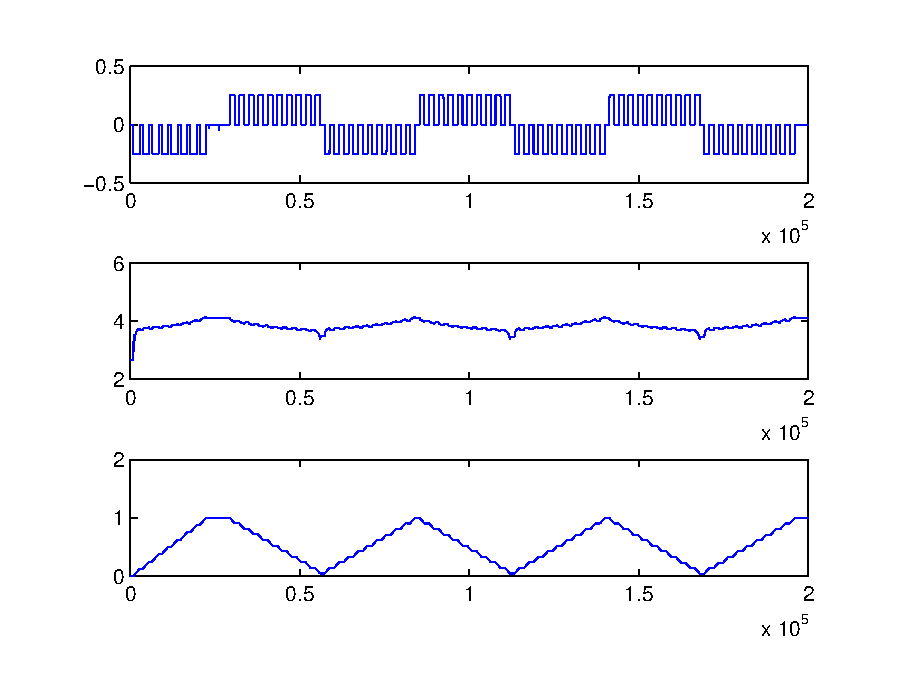
\includegraphics[width=0.9\textwidth]{sim_ideal}
%\caption{Discharge current along with the resulting voltage and SOC.}
%\label{fig:idealsim}
%\end{figure}

\end{document}
